\documentclass[11pt]{article}
\usepackage{preprint}

\usepackage{amsmath, bm}
\usepackage{mathtools}   % for \coloneqq
\usepackage{amssymb} % in preprint.sty
\usepackage[capitalise, noabbrev]{cleveref}
\usepackage{graphicx}
\usepackage{wrapfig}

% todo stuff
\usepackage{soul}
\usepackage{todonotes}
\newcommand{\hlfix}[2]{\texthl{#1}\todo{#2}}

% Colors
\definecolor{accent}{HTML}{004074}   % AGU navy
\newcommand{\red}[1]{\textcolor{red}{#1}}

% References
\usepackage[authoryear, round]{natbib}
\bibliographystyle{abbrvnat}

% ================================================================
%  Title block metadata
% ================================================================
\shorttitle{Nested-EAGLE}
\title{Nested-EAGLE: A Data Driven Global Weather Model with High
Resolution over the Contiguous\\United States}

\authors{%
    Timothy A. Smith\textsuperscript{1,2,*},
    Mariah Pope\textsuperscript{3},
    Sergey Frolov\textsuperscript{1},
    Brett Basarab\textsuperscript{1, 4},
    Daniel Abdi\textsuperscript{4, 5},
    Isidora Jankov\textsuperscript{5},
    Bo Huang\textsuperscript{1, 4}
}

\affiliations{%
    \textsuperscript{1}Physical Sciences Laboratory (PSL), National Oceanic and
        Atmospheric Administration (NOAA), Boulder, CO, USA\\
    \textsuperscript{2}Nansen Environmental and Remote Sensing Centre,
        Bergen, Norway\\
    \textsuperscript{3}Earth Prediction Innovation Center (EPIC)\\
    \textsuperscript{4}Cooperative Institute for Research in Environmental Sciences
        (CIRES) at the University of Colorado Boulder, Boulder, CO, USA\\
    \textsuperscript{5}Global Systems Laboratory (GSL), National Oceanic and
        Atmospheric Administration (NOAA), Boulder, CO, USA
}
\email{timothy.smith@nersc.no}

% ================================================================
\begin{document}
% ================================================================

\maketitle

% ----------------------------------------------------------------
\begin{abstract}
    NOAA’s suite of Numerical Weather Prediction systems spans a wide range of
    spatiotemporal scales. Each forecast system within the suite is uniquely
    tailored to its application, with tuned physical parameterizations and model
    resolutions relevant to the situation. While some separation between
    different modeling systems is practical, computational resource constraints
    generally prohibit forecast systems from using high resolution to forecast
    for long lead times.
    Here, we present a forecast model that takes an ``all in one'' approach,
    leveraging advancements in Machine Learning Weather Prediction (MLWP). Building
    on work from Met Norway, the model operates on a quarter degree resolution
    globally, with a 6 km refinement over the contiguous United States, using
    training data from NOAA’s archives of Global Forecast System (GFS) and the
    regional High Resolution Rapid Refresh (HRRR) analysis. We present an evaluation
    of the model’s forecast skill compared to archived HRRR and GFS forecasts. In
    terms of Mean Squared Error (MSE), the neural network generally outperforms GFS
    and HRRR up to about 10 days, with significant skill gain in the near surface
    and low-level atmosphere. Thus, the model shows promise at providing the best of
    both worlds, capturing both the short and medium range timescales accurately.
    However, we also show a quantitative analysis of precipitation prediction skill,
    which exposes shortcomings in terms of its ability to represent precipitation
    patterns. The assessment motivates future work in order to improve the
    representation of precipitation extremes, including the injection of
    stochasticity into the model along with a variance-penalty loss term, or a
    feature-based loss.

\end{abstract}
% ----------------------------------------------------------------

\section{Introduction}

% NOAA prediction suite
The National Oceanic and Atmospheric Administration (NOAA) regularly broadcasts
weather and climate forecasts to the public for a variety of applications,
for example
severe thunderstorms,
hurricanes,
10 day weather,
and seasonal outlooks of temperature and precipitation.
While significant effort has developed a unified modeling framework
from which prediction systems can be developed \citep{jacobs_open_2021},
there is no ``single'' forecast system at NOAA.
Rather, there are many distinct forecasting systems made up of model and data
assimilation frameworks tuned to the application at hand.
While some separation is both practical and necessary,
e.g., it does not make sense to run a moving nest hurricane model outside of
hurricane season,
forecasters could benefit from a single prediction system that reliably
simulates across multiple scales, and obviates the need to collect results from numerous
systems.

% Hone in on SRW and MRW
We are specifically focused on jointly predicting short range weather,
spanning hours to a few days,
and medium range weather, which generally extends to about two weeks.
At NOAA, short range weather is currently captured by the High Resolution Rapid Refresh
(HRRR): a limited area model (LAM) covering the Contiguous United States (CONUS)
that provides forecasts every hour out to 18~hours at 3~km spatial resolution
\citep{dowell_high-resolution_2022}.
On the other hand, medium range weather is provided by NOAA's Global Forecast
System (GFS) and Global Ensemble Forecast System (GEFS) for deterministic and
stochastic predictions, initialized every 6~hours and released at 0.25$^\circ$
(operating at 13~km as of v16) \citep{noaa_emc_nfs}.
\hlfix{
    Traditional approaches to combining these systems would involve the development
of a single physical simulator, with a nested or refined high resolution mesh
over CONUS.
However, approaches like this are extremely challenging demanding, as there are
$\mathcal{O}(10^8)$ degrees of freedom and the system is
bottlenecked by the Courant-Friedrichs-Lewy condition.
}{bit of a strawman}
The computational load of traditional systems like this limit its
practicality, as the compute time can take longer than the horizon for which the
short range forecast is useful.

% ML offers the opportunity to do this
Developments in machine learning weather prediction (MLWP)
offer an alternative approach to the problem.
In recent years, a number of MLWP models trained on the
ERA5 \citep{hersbach_era5_2020}
have been developed that are competitive with the gold
standard in medium range weather:
the deterministic IFS HRES \red{CITE HRES} and stochastic IFS ENS
\red{CITE ENS} see
\citep{bi_accurate_2023,lam_learning_2023,chen_fuxi_2023,chen_operational_2025,bodnar_foundation_2025,lang_aifs_2024,sadeghi_tabas_gfs-powered_2025}.
Since the development of global, medium range MLWP models, regional weather
emulators have taken off
\citep[e.g.,][]{adamov_building_2025,flora_wofscast_2025,abdi_hrrrcast_2026}.
Notably, \citet{nipen_regional_2026} develop an ``all-in-one'' MLWP model
that has high (2.5~km) resolution over Scandinavia, but still captures the rest
of the globe at $0.25^\circ$.
After a pretraining phase on ERA5 data,
the model is trained on a combination of data from the LAM and global forecast
archives, resulting in state-of-the-art prediction skill out to 2.5~days
at a fraction of the computational cost compared to the traditional system
(ignoring training costs).

% Now introduce Nested-EAGLE
Here, we build on the work by \citet{nipen_regional_2026} to develop
Nested-EAGLE: a MLWP with a high resolution (6~km) mesh over CONUS, nested
inside a $0.25^{\circ}$ grid.
Trained on NOAA's HRRR and GFS analysis\todo{define DA analysis} archives, the model
achieves state-of-the-art prediction skill over CONUS, gaining approximately
2~days of skill over the HRRR and GFS forecast systems.
Aside from distinctly different geographical foci as well as some technical design choices,
we extend the evaluation protocol considered by \citet{nipen_regional_2026} for a nested or
``stretched-grid'' model.
Specifically, our unique contributions are as follows.
\begin{itemize}
    \item We evalute the model at both short and medium range timescales, i.e.,
        out to 15~days.
    \item We highlight the model's skill outside of CONUS to show that the model
        remains a competitive medium range weather model, and is not overtrained
        on our region of choice.
    \item We compare perturbation experiment results to highlight the state variables
        that benefit most from combining HRRR and GFS data during training, and
        isolate the effects of training data. \todo{bias correct..}
    \item To facilitate all of these comparisons and highlight the benefit of
        incorporating HRRR data into Nested-EAGLE, we include comparisons to a single
        resolution (0.25$^\circ$) baseline model trained on GFS analysis data
        only, but using otherwise a mirrored model architecture.
\end{itemize}
Finally, we highlight the model's current weaknesses in representing
precipitation due to the known blurring effect of deterministic ML training at
6~hour timesteps using a mean squared error loss function
\citep[e.g., as noted by][]{lam_learning_2023}.
However, we provide a nuanced view that offers hope for future development.

\section{Prognostic Forecast Skill}
\label{sec:prognostic_skill}

We evaluate the performance of Nested-EAGLE over the test period,
February 2024--January 2025 by comparing its forecast skill against the relevant physics based modeling
frameworks from NOAA: GFS and HRRR.
In our prognostic skill evaluation,
e.g., for 2m temperature,
we compare 15~day forecasts initialized every 30~hours, evenly sampling the
diurnal and seasonal cycles during the period while resulting in 293~samples per
lead time.
Forecasts from each model are evaluated in terms of Root Mean Squared Error
(RMSE) against in situ observations,
e.g., dropsondes, rawinsondes, aircraft, and station data,
from the NOAA NASA Joint Archive \citep[NNJA;][]{nnja_obs_data} via Brightband's
Python API \citep{hans_mohrmann_2025_16749100}.
We note that conducting the evaluation against observations was critical,
because the model combines analysis states from both GFS and HRRR.
Comparing against observations allows us to control for regions in the analyses
which are different from each other, but unconstrained by data.
See \red{Supplement} for details, comparing separate evaluations against
observations and HRRR analysis.

\subsection{Forecast Skill Over CONUS}
\label{subsec:conus_skill}

\begin{figure}[t]
    \centering
    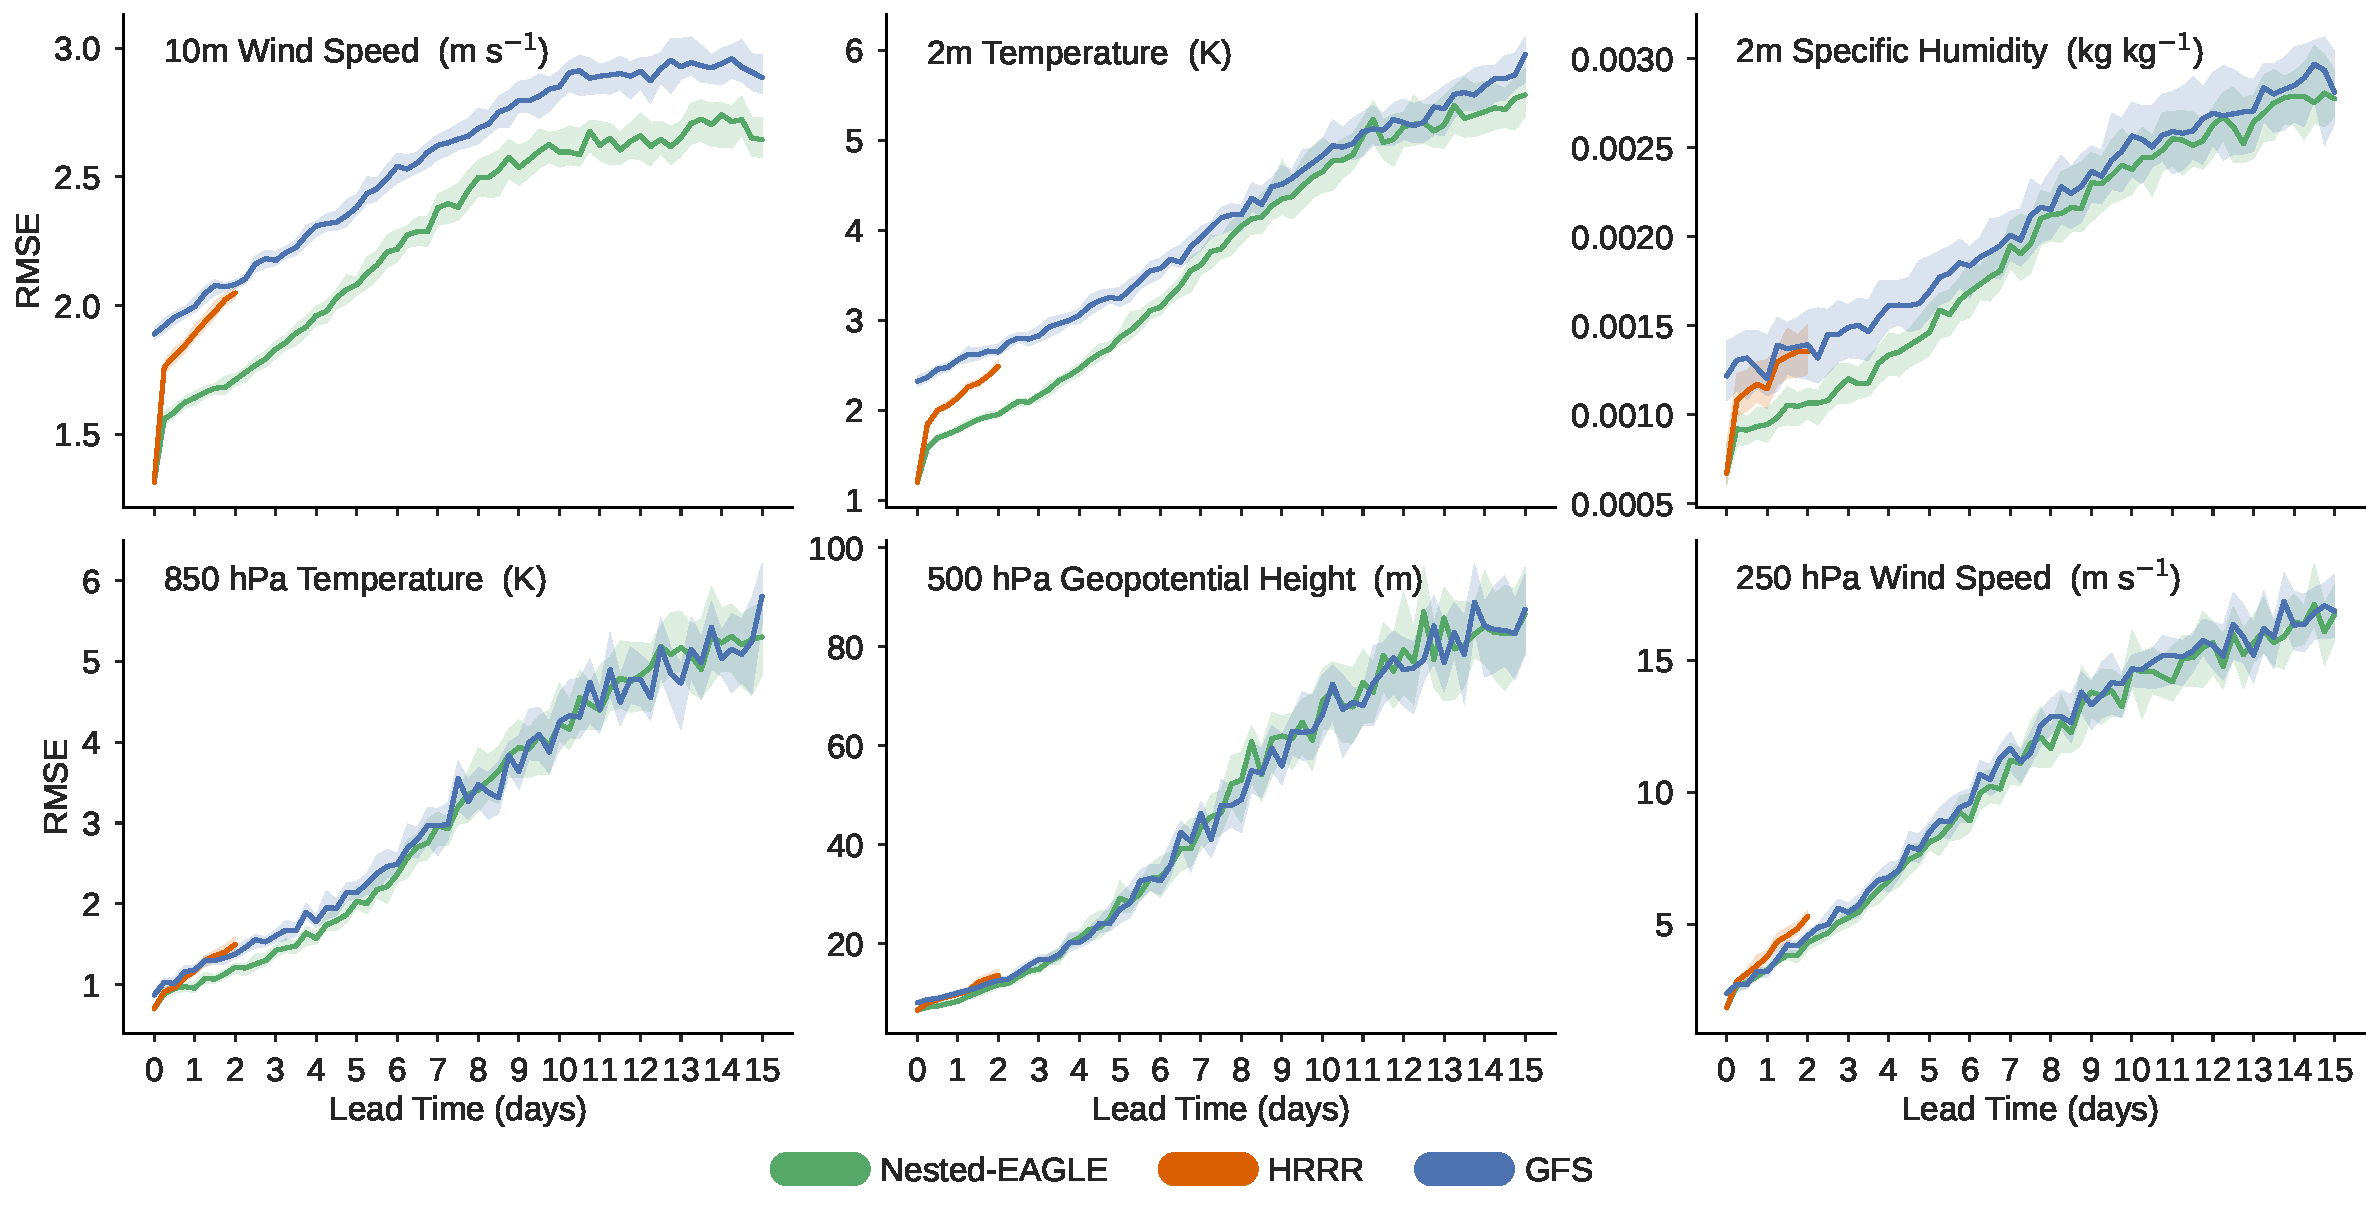
\includegraphics[width=\textwidth]{figures/lam_rmse.pdf}
    \caption{
        \textbf{
            RMSE against in situ observations over CONUS from Feb. 2024--Jan. 2025 for select
            quantities.
        }
        Dark solid lines indicate the mean over 293~forecasts initialized every
        30~hours, and shading indicates the 95\% confidence interval.
        The model forecasts are first conservatively regridded to the same 6~km resolution
        grid that Nested-EAGLE employs over CONUS, then bilinearly interpolated to the
        observation locations.
    }
    \label{fig:lam_rmse}
\end{figure}

\cref{fig:lam_rmse} shows that Nested-EAGLE generally has the lowest mean error over
CONUS, especially for near surface quantities, and remains competitive
throughout the atmosphere to 15~days.
More specifically, \cref{fig:lam_rmse} shows RMSE for Nested-EAGLE, HRRR, and
GFS for the longest lead time available from each forecast model.
The top row shows a selection of near surface variables, for which Nested-EAGLE
maintains a \red{roughly two day} lead in skill.
This skill gap closes at roughly 5--7~days for 2m~temperature and
2m~specific humidity, at which point the mean error from Nested-EAGLE is
statistically indistinguishable from GFS, assuming a 95\% confidence interval.
The bottom row of \cref{fig:lam_rmse} shows RMSE for a selection of fields
indicating skill across the atmospheric column.
At 850~hPa, Nested-EAGLE maintains a statistically significant
$\sim$1~day\todo{check this}
lead in temperature skill over HRRR and GFS, although this is relatively muted compared to
the near surface variables.
Higher up into the atmosphere, for example as shown by 500~hPa geopotential
height and 250~hPa wind speed errors, Nested-EAGLE and GFS show essentially the
same skill.

The reason that Nested-EAGLE leads in surface quantities, but only remains
competitive in the upper atmosphere is purely due to differences between the
HRRR and GFS analysis states, i.e., the state at forecast hour 0.
For near surface variables, HRRR analysis leads the GFS analysis by a
significant margin: approximately 0.75~m~s$^{-1}$\todo{check} \red{convert to
percentage}.
We presume that these near surface improvements are due to several factors in
the HRRR data assimilation system, including:
(1) higher spatial resolution,
(2) more frequent assimilation cycles (hourly versus 6~hourly),
(3) a more advanced land model, which can make better use of surface
observations,
and (4) better observational coverage, using more US centric station data.
On the other hand, differences in the atmospheric fields shown in the bottom row
of \cref{fig:lam_rmse} are between \red{X\%--Y\%}.
That is, HRRR and GFS have approximately the same atmospheric state, but HRRR
translates this representation into a better surface state.
We note that the relative improvements near the surface are not due to scaling
the loss function to prioritize the surface and deprioritize the atmosphere,
for example which is used by
GraphCast \citep{lam_learning_2023} and AIFS \citep{lang_aifs_2024}.
In fact, we found this scaling to be detrimental to skill across all variables
\red{Ref Supplement}.
Thus, Nested-EAGLE's skill gain for near surface quantities is due to the
propagation of skill gains in the HRRR analysis, indicating the benefit of
incorporating the data into training.

\subsection{Forecast Skill Over Europe}
\label{subsec:europe_skill}

\begin{figure}[t]
    \centering
    \includegraphics[width=\textwidth]{figures/europe_rmse.pdf}
    \caption{
        \textbf{
            RMSE against in situ observations over Europe from Feb. 2024--Jan. 2025 for select
            quantities.
        }
        Dark solid lines indicate the mean over 293~forecasts initialized every
        30~hours, and shading indicates the 95\% confidence interval.
        The Europe region is defined as a latitude-longitude box from
        35$^\circ$N--75$^\circ$N and 25$^\circ$W--65$^\circ$E.
        All datasets operate on a 0.25$^\circ$ latitude-longitude grid in this
        region, and no regridding is performed for the evaluation.
    }
    \label{fig:europe_rmse}
\end{figure}

\cref{fig:europe_rmse} shows that outside of the target region, CONUS,
Nested-EAGLE does not carry over skill learned from the HRRR dataset, but
still remains a reliable medium range weather model.
The figure shows RMSE against in situ observations over Europe, comparing
Nested-EAGLE, GFS, and a single resolution MLWP model baseline that is trained
on GFS analysis data only.
Outside of the US, Nested-EAGLE and the ML baseline produce statistically
identical results.

This result provides a ``gut check'' for Nested-EAGLE.
While it would be ideal for Nested-EAGLE to carry over skill gains from the HRRR
dataset to the rest of the globe, the model is trained with a
supervised learning objective that essentially prohibits it from doing so
because the target data outside of CONUS is defined by GFS analysis.
It is therefore reassuring that the model is not overtrained to its target region, and
remains a reliable global model as well.
We note that most nested or stretched-grid ML models reweight the loss function
to give the target region higher priority (Bris: X, West: Y, Paper: Z), whereas
our tuning indicates a more moderate 10\% works best for our targe region \red{see Supplement}.
More moderate values could be important for skill outside of the target
region.\todo{discussion? useful?}

\subsection{Learned Constraints or Errors of the Day?}
\label{subsec:ic_experiment}

The previous sections show that incorporating HRRR analysis into global MLWP model
training improves its representation of near surface quantities over CONUS.
However, a fundamental limitation of Nested-EAGLE, and most of the MLWP models
from the broader community, is its reliance on an analysis state
that comes from traditional data assimilation systems.
% Leave this until discussion time
%generally provided
%publicly by operational centers like NOAA or ECMWF.
In our framework, which nests the HRRR analysis inside of GFS analysis, it is
not exactly clear \textit{how} the skill gain manifests.
Are the skill gains in Nested-EAGLE relative to the ML baseline purely due
to the fact that we feed it
an improved initial state at inference time, or are the improvements baked into
the model during training?

\begin{figure}[t]
    \centering
    \includegraphics[width=\textwidth]{figures/swapped_ic_rmse.pdf}
    \caption{
        \textbf{
            RMSE over CONUS, similar to \cref{fig:lam_rmse}, but with additional
            experiments perturbing initial conditions.
        }
        The additional purple dashed line shows the RMSE of Nested-EAGLE when it
        is initialized with GFS data only at inference time.
        The brown dashed line shows the opposite: the ML baseline, which is
        only trained on GFS analysis, is fed initial conditions that have HRRR
        data over CONUS.
        Dark solid lines indicate the mean over 293~forecasts initialized every
        30~hours, and shading indicates the 95\% confidence interval.
        All datasets are conservatively regridded to a 0.25$^\circ$ resolution
        and evaluated over an approximate CONUS latitude-longitude box from
        20$^\circ$N--55$^\circ$N and 135$^\circ$W--50$^\circ$W.
    }
    \label{fig:ic_experiment}
\end{figure}


\cref{fig:ic_experiment} shows that the improvements are learned during
training, and carry over even with \red{degraded} initial conditions.
Similar to the top row of \cref{fig:lam_rmse}, \cref{fig:ic_experiment} shows
near surface forecast RMSE over CONUS from Nested-EAGLE, GFS, and
the single resolution ML baseline.
Additionally, \cref{fig:ic_experiment} shows the skill when Nested-EAGLE is
initialized with only GFS analysis at inference time (purple dashed line).
We note that in order to make the Nested-EAGLE mechanics work,
the GFS state is conservatively interpolated to the 6~km Lambert Conic Conformal
grid over the HRRR subdomain, and left ``as-is'' over the rest of the globe.
Conversely, \cref{fig:ic_experiment} also shows the skill when the ML baseline,
trained only on GFS analysis data, is given HRRR initial conditions at
inference time (brown dashed line).
Similarly, for the mechanics to work with the single resolution model,
the HRRR state is conservatively coarsened to a 0.25$^\circ$ degree
latitude-longitude projection, and swapped into the global grid as appropriate.
In \cref{fig:ic_experiment}, models initialized with swapped
analysis states start with the appropriate errors; for example,
Nested-EAGLE-Swapped has the same error as GFS at forecast hour 0.
However, the two swapped models rapidly converge to the
same error as models that use consistent initial conditions during training and inference.
For 10~m wind speed, this convergence essentially happens in the first 6~hour
time step.
For 2~m temperature, the ML baseline with GFS and HRRR initial conditions
loses skill almost immediately as well, whereas Nested-EAGLE with GFS-only
initial conditions takes slightly longer to converge (although still only 24--36~hours).
The slower convergence appears to be mostly due to orography.
In addition to swapped model states, Nested-EAGLE-Swapped
uses GFS orography, and the remaining differences between Nested-EAGLE and
Nested-EAGLE-Swapped correspond to a lapse rate
that correlates with elevation errors between GFS and HRRR \red{Supplement}.


Visualizing the spatial distribution of errors between Nested-EAGLE and
its swapped counterpart shows that it has learned to remove errors from the GFS
analysis.
That is, \cref{fig:nested_swapics_spatial_rmse}
shows spatial maps of RMSE between Nested-EAGLE and Nested-EAGLE-Swapped,
averaged over the forecasts from the test period.
Within the first 6~hour time step, large errors over the Great Plains and near
the coastlines are removed.
By 30~hours into the forecast, the only notable differences between the two
experiments are in the 2m~temperature field over regions with high elevation,
where persistent biases remain owing to orographic differences noted earlier.
However, these differences are small relative to the initial error
between GFS and HRRR analysis.

\begin{figure}[t]
    \centering
    \includegraphics[width=\textwidth]{figures/nested_swapics_spatial_rmse.jpeg}
    \caption{
        \textbf{
            Spatial RMSE between Nested-EAGLE and Nested-EAGLE-Swapped, averaged
            over the 293~forecasts from Feb. 2024--Jan. 2025.
        }
        At forecast hour 0 (left column), differences are entirely due to
        differences in GFS and HRRR analyses.
        After 6~hours (middle column), the figure shows the difference between Nested-EAGLE with
        and without HRRR data over CONUS after a single forecast step.
        By 30~hours (right column), the differences are negligible.
    }
    \label{fig:nested_swapics_spatial_rmse}
\end{figure}

\section{Precipitation Evaluation over CONUS}
\label{sec:precip}

Similar to the prognostic skill evaluation presented in
\cref{sec:prognostic_skill}, we evaluate Nested-EAGLE's ability to predict
6~hour accumulations of precipitation as a function of forecast hour
during February 2024--January 2025.
However, we employ a different evaluation protocol for precipitation compared to
the other fields.
Most importantly, we focus on the Fractions Skill Score
\citep[FSS;][]{roberts_scale-selective_2008} metric, which emphasizes spatial
coherency and gives better scores to models that predict precipitation
fields that ``look like'' observations \red{See supplement/methods}.
We compare 1426~forecasts from each model,
generated from forecasts initialized every 6~hours during the test period.
Because it is challenging to find high resolution, high quality observational
estimates of precipitation across the globe that provide an independent
reference, we limit our evaluation to the CONUS region,
using NOAA's Analysis of Records for Calibration
\citep[AORC;][]{fall_aorc_2023} as a reference.
All datasets are conservatively regridded to the 6~km resolution of Nested-EAGLE
over CONUS, such that the total precipitation amounts are preserved.
Finally, the hourly AORC data is aggregated so that all datasets show
6~hour accumulations.

\subsection{Precipitation Skill per Amount}
\label{subsec:fss_threshold}

%\begin{wrapfigure}{r}{0.62\textwidth}
\begin{figure}
    \centering
    \includegraphics[width=.6\textwidth]{figures/fss_threshold_conus.pdf}
    \caption{
        \textbf{
            FSS over CONUS during Feb. 2024--Jan. 2025, using AORC as the
            reference, shown as a function of the threshold quantity.
        }
        All datasets were conservatively regridded to the same 6~km resolution
        that Nested-EAGLE uses over CONUS, and the AORC dataset was aggregated
        from hourly to 6~hourly accumulations.
        A value of 1 indicates a perfect FSS, i.e., higher is better.
    }
    \label{fig:fss_threshold_conus}
%\end{wrapfigure}
\end{figure}

\cref{fig:fss_threshold_conus} quantifies the most central limitation of
Nested-EAGLE: precipitation amplitudes are weak relative to the physical model
baselines.
That is, each panel shows how well each model represents a given amount of
precipitation accumulated over the most recent 6~hours,
with panels indicating skill at 6~hours and 24~hours of lead time.
While all models are less skillful at higher thresholds, HRRR is clearly the
most skillful forecast model at all threshold levels, except for the smallest
thresholds (1--2 mm$/6$h) where
Nested-EAGLE has a slight advantage.
At 6~hours of lead time, Nested-EAGLE FSS is nearly identical to the
archived 0.25$^\circ$ GFS forecasts, despite operating at 6~km spatial
resolution.
FSS from all models degrades with lead time, and this is slightly more dramatic
for Nested-EAGLE at the 20--60 mm$/6$h range.

The reason Nested-EAGLE produces weak amplitudes relative to its
resolution is due to its deterministic training with a MSE loss function.
More specifically, the MSE loss function suffers from the double-penalty effect
\citep{rossa_overview_2008},
leading to predictions that blur the small scale features
\citep[as noted by many, e.g.,][]{lam_learning_2023}.
The relatively blurred small scales result in diminished local maxima, and
reduced skill at higher precipitation thresholds.

\subsection{Precipitation Skill per Percentile}
\label{subsec:fss_percentile}

%\begin{wrapfigure}{r}{.62\textwidth}
\begin{figure}
    \centering
    \includegraphics[width=.6\textwidth]{figures/fss_percentile_conus.pdf}
    \caption{
        \textbf{
            Same FSS scores as \cref{fig:fss_threshold_conus}, except shown as a function
            of percentile represented by each model.
        }
        All datasets were conservatively regridded to the same 6~km resolution
        that Nested-EAGLE uses over CONUS, and the AORC dataset was aggregated
        from hourly to 6~hourly accumulations.
        A value of 1 indicates a perfect FSS, i.e., higher is better.
    }
    \label{fig:fss_percentile_conus}
\end{figure}
%\end{wrapfigure}

Despite the blurring imposed by deterministic training,
\cref{fig:fss_percentile_conus} shows some nuance in the
evaluation, indicating that Nested-EAGLE can still represent the location of
precipitation events well.
In \cref{fig:fss_percentile_conus}, FSS is shown as a function of the percentile
that each model is able to represent.
At 6~hours of lead time, Nested-EAGLE and HRRR are the most skillful,
with indistinguishable FSS per percentile.
The fact that the two curves match is reassuring, because the 0--6~hour
accumulation from HRRR is used as targets for Nested-EAGLE during training.
All models show degraded FSS with increasing lead time in the percentile view,
but the rankings change amongst models.
At 24~hours of lead time, Nested-EAGLE is the most skillful across all
percentiles, and GFS surpasses HRRR at thresholds below the 80$^\text{th}$ percentile.

We surmise that HRRR's reduced skill, at least when viewed in this percentile
framing, is due to the challenging nature of capturing the
location of lower likelihood events at longer lead times with deterministic,
high resolution physical forecast systems.
As lead time extends, HRRR departs from the initial condition constraints
provided by data assimilation, and tends toward the numerical model's attractor,
which is distinctly different from the observations.
On the other hand, Nested-EAGLE is trained to produce HRRR's 0--6~hour
precipitation accumulation at all lead times, which is the 6~hour accumulation
most constrained by data assimilation.
While the ML model will tend toward its own attractor, distinct from HRRR's 0--6~hour
accumulation, it appears to maintain its own
representation of the lower likelihood events better than the physical models.

\section{Discussion}
\label{sec:discussion}

Weather forecast accuracy depends upon the ability of numerical weather
prediction systems to represent dynamics across a wide range of spatiotemporal
scales.
While \red{it would be convenient to provide} a single high resolution forecast for
multiple weeks,
computational constraints of traditional, physics-based prediction systems
necessitates providing separate forecasts for distinct spatiotemporal ranges.
Advances in MLWP provide alternatives which may bend these constraints.
Toward this end, we presented Nested-EAGLE: a MLWP that seamlessly forecasts short and
medium range weather over CONUS.
When compared against in situ observations, the model leads NOAA's current operational
forecast systems for key quantities like 2m temperature and 10m wind speed
by roughly \red{2 days} of forecast skill, for at least \red{5 days} of lead.
We showed that this skill stems from HRRR analysis data, and has the largest
benefits for near surface quantities.
However, given that HRRR forecasts only extend to a maximum of 48~hours, Nested-EAGLE
can be taken as an improvement to \red{the status quo} because it readily extends that
predictability into the medium range.

Outside of CONUS, we showed that Nested-EAGLE performs similarly to a global
MLWP model, providing reliable medium range forecast scores.
While it would be ideal for improvements from the HRRR dataset to allow for
improved skill elsewhere, the current supervised training regiment essentially
prohibits this --- Nested-EAGLE can only be as good as the data provided at its
particular location.
This evaluation shows that the model is not overfit to its target region, and we
note relevant ablation experiments which could be useful to other operational
centers that are now developing nested or ``stretched-grid'' MLWP models.
More importantly, these tests show the importance of accurate training data
during supervised learning.

We tested the impact of providing Nested-EAGLE GFS initial conditions only,
interpolating the data as if it were the 6~km coarsened HRRR analysis used
normally.
With these initial conditions, Nested-EAGLE produces forecasts that are nearly
as accurate as when the typical HRRR/GFS data are used.
Spatial analysis showed that the model acts as a sort of bias
corrector, removing errors along the Great Plains and coastlines
from the GFS initial conditions rapidly.
Taken together, these experiments confirm that
Nested-EAGLE's skill is not due to better initial conditions at inference time,
but rather learned during training time.
There are several implications from this finding.
On the one hand, Nested-EAGLE is robust to degraded initial conditions,
perhaps due to missing observational constraints during the data assimilation
phase.
However, these experiments also imply that improved initial conditions, for
example due to a system upgrade or increased observations, would not immediately
benefit the model at forecast time.
Instead, within the framework shown here, improved initial conditions need to be
incorporated into training for the benefits to be realized by the ML model.
Thus, our results motivate future work to incorporate observations into the
model training directly.
Most immediate work could add observational constraints to the loss
function, which would sidestep the need to nest or otherwise combine analyses
based on their skill for a given region.
More generally though, future work should consider modeling frameworks that
operate on observational inputs directly in order to more directly respond to
improved observational constraints.
New advancements in ``end-to-end'' ML forecasting \citep{pinnington_aifs-dop_2026}
and ML state estimation \citep{gupta_healda_2026} offer promise for these
directions.

In a separate analysis of precipitation forecast skill, we showed that
Nested-EAGLE's representation of precipitation is comparable to GFS, despite
operating at a higher 6~km resolution.
The results show a quantification of the blurring effect that a MSE-based loss
function imparts on MLWP models during training.
These results motivate future work to improve the spatial representation in the
model.
Considering results by
\citet{nordhagen_high-resolution_2025,lang_aifs-crps_2026,alet_skillful_2025,bonev_fourcastnet_2025},
we suggest that training a stochastic model with a Continuous Ranked Probability
Score loss function would be a fruitful first step, for both spatial and more
explicit uncertainty representation.
\red{CITE Canada? Subich paper?}

Moreover, viewing Nested-EAGLE's precipitation FSS in terms of percentiles
indicates that the model accurately predicts the position of precipitation
events, despite blurring the amplitudes.
This finding is analogous to prior work, showing that deterministic global MLWP
models accurately capture hurricane storm track, despite underestimating
intensity \red{CITE HURRICANE}.
Our hope is that future versions of Nested-EAGLE can improve spatial
representation, while still maintaining the positional accuracy.
At longer lead times, Nested-EAGLE is shown to produce the most accurate
precipitation forecast on a percentile basis.
Our assumption is that this advantage is due to the fact that Nested-EAGLE is
trained on HRRR forecasts that are still highly constrained by data
assimilation.
If true, \red{this implies} that incorporating observations would lead to even
better predictions at longer lead times, side stepping the bounds of
predictability bounds of a forecast model.
Initial exploration by \red{CITE Met Norway} indicate that this line of work is
fruitful, but remains an open challenge.

Nested-EAGLE is one of many exploratory MLWP models being tested at NOAA,
alongside its global \citep{sadeghi_tabas_gfs-powered_2025} and
LAM \citep{abdi_hrrrcast_2026} counterparts.
The model is currently producing forecasts for 2026 in a quasi-operational
environment, with forecasts to be published soon.


% ----------------------------------------------------------------
%  References
% ----------------------------------------------------------------
\bibliography{references}

% ================================================================
\end{document}
